\chapter{Related Work}
\section{Embedded Databases}
\subsection{DuckDB}
DuckDB is an in-memory, embedded, columnar, OLAP Database\cite{DuckDBPaper} developed as a successor to MonetDBLite\cite{MonetDBLitePaper} in the embeddable database OLAP niche.
\begin{center}
    \begin{tabular}{l p{.8\textwidth}}
        \textbf{Embedable}         & The database is a single file with no dependencies, and is easily embeddable in and usable from applications written in Python, R, Java, Julia, Swift and Rust\cite{DuckDBDocs}. \\
        \textbf{Cost-Aware}        & In addition to common rule-based optimisations, DuckDB uses a cost-model and statistics collected at runtime for its logical optimizer.                                          \\
        \textbf{Extensible}        & DuckDB supports loadable WASM extensions.                                                                                                                                        \\
        \textbf{Language Agnostic} & DuckDB communicates through the C-ABI and uses its heap, as a result it cannot take advantage of language/compiler specifics (e.g. data representation).                         \\
        \textbf{Columnar}          & To better support OLAP access patterns. This hurts OLTP performance, which is better suited to a nary storage, furthermore the only supported indexes are zonemaps/min-max
        indexes and adaptive radix trees. Neither offer lookup performance comparable to hash indices.                                         \\
        \textbf{Concurrency}       & DuckDB uses a combination of optimistic and multiversion concurrency control.                                                                                                    \\
    \end{tabular}
\end{center}
\noindent
\subsubsection{System Design}
The authors describe the design as \textit{"textbook"}\cite{DuckDBPaper}.
\begin{figure}[h!]
    \centering
    \includegraphics[scale=1]{related_work/_diagrams/duckdb_system.pdf}
    \caption{An overview of the DuckDB system design.}
\end{figure}
\subsubsection{Vector Volcano Processing}
DuckDB uses a \textit{vector volcano} processing model. The interpreter takes a dynamically constructed tree of operators, wherein each operator pulls data from input operators on demand much like with volano processing.
However instead of pulling individual tuples, \mintinline{Cpp}{DataChunks} are passed, each containing a tuple of column vectors for a row-range of the previous operator's output.
\begin{center}
    \includegraphics[scale=1]{related_work/_diagrams/duckdb_operators.pdf}
\end{center}


\subsection{SQLite}
SQlite is a lightweight embedded database\cite{SQLitePaper}, and is currently the most deployed database in the world\cite{SQLiteWebsite}.
Unlike DuckDB it is designed for OLTP workloads, and as such stores rows in an nary record format.
\subsubsection{System Design}
\begin{figure}[h!]
    \centering
    \includegraphics[scale=1]{related_work/_diagrams/sqlite_system.pdf}
    \caption{An overview of the SQLite system design.}
\end{figure}

\subsubsection{Virtual Database Engine Bytecode}
One of the key elements of SQLite's design is that rather than using traditional physical plan (i.e. trees of operators) it instead uses a simple bytecode, interpreted on the virtual database engine.
\begin{minted}{SQL}
CREATE TABLE users (
    id INTEGER PRIMARY KEY AUTOINCREMENT,
    name VARCHAR NOT NULL,
    premium BOOLEAN NOT NULL,
    credits MEDIUMINT NOT NULL,
    CONSTRAINT premcredits CHECK (premium OR credits >= 0)
);

-- Get Total Premium credits
EXPLAIN SELECT SUM(credits) FROM users WHERE premium = TRUE;
\end{minted}
When run with SQLite (compiled with \mintinline{bash}{-DSQLITE_ENABLE_EXPLAIN_COMMENTS}) the following bytecde is returned:
\begin{center}
    \begin{tabular}{l l | l l l l l | l}
                      &                 & \multicolumn{5}{c|}{\textbf{Registers}} &                                                                                                               \\
        \textbf{addr} & \textbf{opcode} & \textbf{p1}                             & \textbf{p2} & \textbf{p3} & \textbf{p4}     & \textbf{p5} & \textbf{comment}                                  \\
        \hline
        0             & Init            & 0                                       & 13          & 0           & null            & 0           & \mintinline{bash}{Start at 13        }            \\
        1             & Null            & 0                                       & 1           & 2           & null            & 0           & \mintinline{bash}{r[1..2]=NULL       }            \\
        2             & OpenRead        & 0                                       & 5           & 0           & 4               & 0           & \mintinline{bash}{root=3 iDb=0; users}            \\
        3             & Rewind          & 0                                       & 9           & 0           & null            & 0           & \mintinline{bash}{               }                \\
        4             & \qquad Column   & \qquad  0                               & \qquad 2    & \qquad 3    & \qquad null     & \qquad 0    & \qquad \mintinline{bash}{r[3]= cursor 0 column 2} \\
        5             & \qquad Ne       & \qquad  4                               & \qquad 8    & \qquad 3    & \qquad BINARY-8 & \qquad 83   & \qquad \mintinline{bash}{if r[3]!=r[4] goto 8   } \\
        6             & \qquad Column   & \qquad  0                               & \qquad 3    & \qquad 3    & \qquad null     & \qquad 0    & \qquad \mintinline{bash}{r[3]= cursor 0 column 3} \\
        7             & \qquad AggStep  & \qquad  0                               & \qquad 3    & \qquad 2    & \qquad sum(1)   & \qquad 1    & \qquad \mintinline{bash}{ accum=r[2] step(r[3]) } \\
        8             & Next            & 0                                       & 4           & 0           & null            & 1           & \mintinline{bash}{              }                 \\
        9             & AggFinal        & 2                                       & 1           & 0           & sum(1)          & 0           & \mintinline{bash}{accum=r[2] N=1    }             \\
        10            & Copy            & 2                                       & 5           & 0           & null            & 0           & \mintinline{bash}{r[5]=r[2]         }             \\
        11            & ResultRow       & 5                                       & 1           & 0           & null            & 0           & \mintinline{bash}{output=r[5]       }             \\
        12            & Halt            & 0                                       & 0           & 0           & null            & 0           & \mintinline{bash}{                  }             \\
        13            & Transaction     & 0                                       & 0           & 3           & 0               & 1           & \mintinline{bash}{usesStmtJournal=0 }             \\
        14            & Integer         & 1                                       & 4           & 0           & null            & 0           & \mintinline{bash}{r[4]=1            }             \\
        15            & Goto            & 0                                       & 1           & 0           & null            & 0           & \mintinline{bash}{              }                 \\
    \end{tabular}
\end{center}

\subsubsection{JIT Compilation for SQLite}
In order to improve performance, without burdening developers with the additional development \& maintenance
cost of writing a JIT compiler, one can be generated from the interpreter. This strategy has been attempted with SQLite\cite{SQLiteJITCompiler} and advertised a $1.72\times$ speedup over a seelction of TPC-H queries.

\section{Code Generation for Databases}
\subsection{Holistic Integrated Query Engine}
The Holistic Integrated Query Engine\cite{HIQUEPaper} is a single-threaded, JIT code generating, general purpose relational database that implements queries using a C++ code generator and attached C++ compiler.
Typical just-in-time compilation powered databases use a lower-level representation, and pass this to a bundled compiler (e.g. LLVM), however there are several advantages to using C++ as the target representation.
\begin{center}
    \begin{tabular}{l p{.8\textwidth}}
        \textbf{Visibility}   & The output is easily inspectable C++, and the compiler can optionally include debug information, or additional instrumentation when compiling queries to assist in debugging the engine, and the compiler itself verifies the type safety of code. While HIQUE was evaluated using GCC, it is possible to swap out the compiler for another (e.g. Clang) for additional features without difficulty. \\
        \textbf{Templates}    & The templates used by the code generator are also written in C++, making them easier to write and maintain.                                                                                                                                                                                                                                                                                          \\
        \textbf{Optimisation} & A broad range of optimisations (including for the native hardware) can be performed, and the compiler has access to the entire context of the query code.
    \end{tabular}
\end{center}
The significant downside to source generation is the time \& system resource taken by using a full C++ compiler, which increases with query complexity, and the level op optimisation. This is particularly problematic for small queries associated with OLTP workloads.
\\
\\ The main focus of HIQUE is to avoid the poor instruction and data cache performance associated with the volcano processing model by using hand-optimised templates to generate cache concious code for common operations. A large focus of this to improve the performance of iteration over rows.
By using the known types of fixed-length tuples, and accessing through direct referencing \& pointer arithmetic, no function calls are required to tuple access, and the system can use the size of the tuple to avoid random accesses to block sizes only resident in the lower levels of the memory hierarchy.
\\
\\ HIQUE also uses a Partitioned Attributed Across (PAX) record layout\cite{PAXStorageModel} that stores fixed size ranges of rows as a tuples of column vectors, this provides the row lookup advantages of nary stprage (all items of a given row are stored in the same page, requiring at most of page load for access), as well as the better cache performance of columnar storage (allowing simple linear scans over columns). This is conceptually similar to the \mintinline{Cpp}{DataChunks} abstraction used by DuckDB.
\subsubsection{System Design}
\begin{figure}[h!]
    \centering
    \includegraphics[scale=1]{related_work/_diagrams/HIQUE_system.pdf}
    \caption{An overview of the HIQUE system design.}
\end{figure}
\subsubsection{Relevance to emdb}
The cost of using a full C++ compiler at compile time is the only major downside to the many upsides of generating high-level code.
\\
\\ By lifting query compilation to the application's compile time, the same benefits can be achieved with emDB, without needing to do any query compilation work at runtime.
\\
\\ The only performance downside of this is that chip-specific parameters (e.g. cache sizes) are only available when the binary is run, if it compiled for an architecture in general, rather than for the exact chip of the machine the application will run on.

\section{Incremental View Maintenance}
\subsection{DBToaster}
\label{sec:db_toaster}
DBToaster is an incremental view maintenance code generation tool, that generates C++, Spark (including a distributed spark target) and OCaml implementations from queries.
\subsubsection{SQL Support}
A SQL syntax is supported (with incomplete compliance with ASNI SQL-92) to construct select queries
on streams\cite{DBToasterSQLReference} of tuple changes and are the only way to write/mutate relations in the system.
Tables are supported, but are static and cannot be modified after load.
\\
\\ By forgoing complex write insert, update and delete queries, DBToaster avoids much of the complexity in combining
transactions, constraints and delta queries (the calculus used for generating delta queries has no support for
relation mutation).
\\
\\ A restricted set of conditionals \& functions are supported, and external functions are possible (depending on backend used).

\subsubsection{System Design}
\begin{figure}[h!]
    \centering
    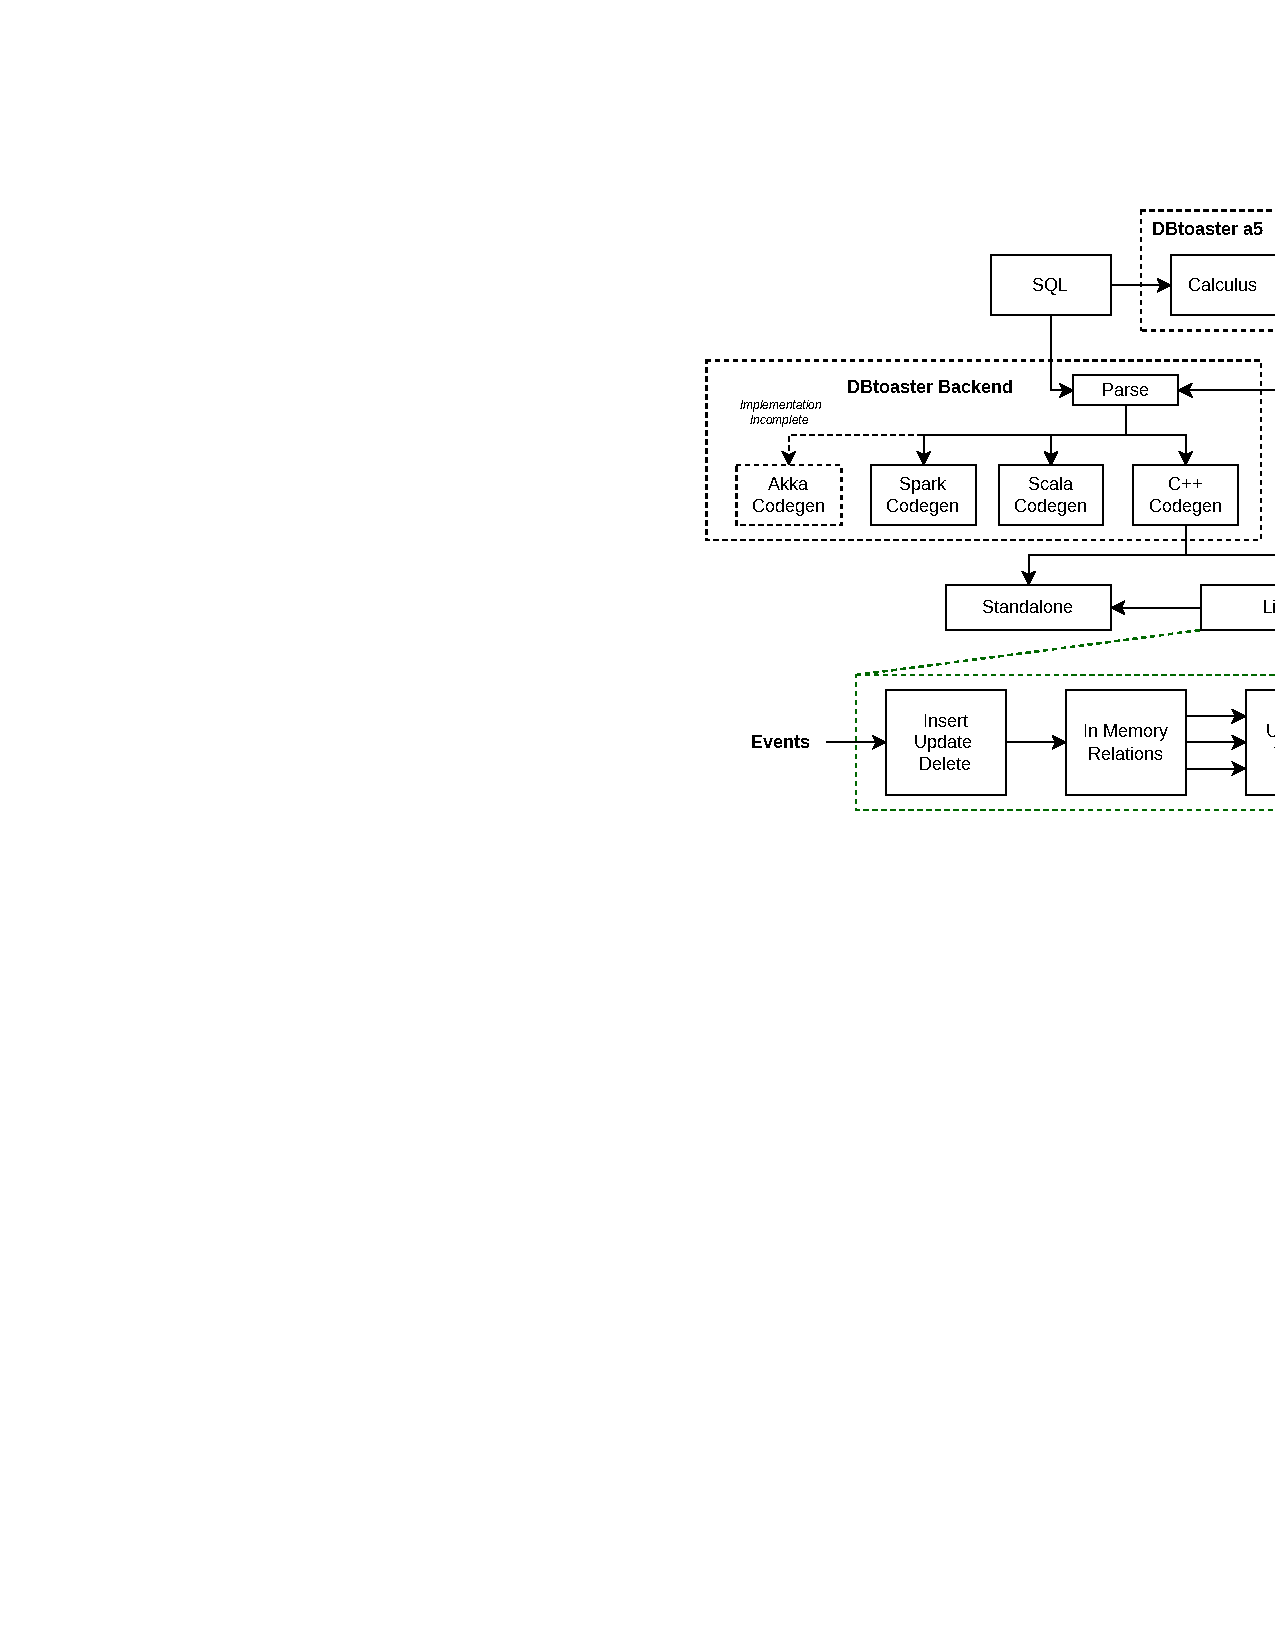
\includegraphics[scale=1]{related_work/_diagrams/dbtoaster_system.pdf}
    \caption{An overview of the DBToaster system design.}
\end{figure}
One of the key advantages for DBToaster is that the code generated is easily embeddable in applications, which provides the same advantages as discussed in \ref{sec:intro_experimentation}.

\subsubsection{Aggregation Calculus}
DBToaster lifts queries parsed from SQL and represented by a simplified relational algebra into its own aggregation calculus (AGCA). AGCA represents data through generalized multiset relations (GMRs) which are mappings from the set of tuples to the multiplicites of those tuples in relations.
\begin{figure}[h!]
    \centering
    
    \includegraphics[scale=1]{related_work/_diagrams/dbtoaster_agca_syntax.pdf}
    \caption{DBToaster AGCA syntax.}
\end{figure}
\begin{figure}[h!]
    \centering
    \includegraphics[scale=1]{related_work/_diagrams/dbtoaster_agca_eval_gmrs.pdf}
    \caption{DBToaster AGCA Generalised Multiset Relations.}
\end{figure}
Evaluation rules for the language are provided in the paper \textit{DBToaster: Higher-order Delta Processing for Dynamic, Frequently Fresh Views}\cite{DBToasterHigherOrderDeltaProcessing} and are ommitted for brevity.
\\
\\ SQL translation is done by converting to relational algebra (with bag semantics), upon which operations can be reduced to union ($+$) and join ($\bowtie$) by judicial allowance for infinite relations. For example $\sigma_{A<B}(R)$ is rewritten as $R \bowtie (A < B)$ despite $A < B$ being an infinitely large set of possible tuples.
\begin{minted}{SQL}
                    SELECT * FROM R WHERE B < (SELECT SUM (D) FROM S WHERE A > C);
\end{minted}
\[Sum_{[A,B]}(R(A,B) \ast (z := Sum_{[]}(S(C<D) \ast (A > C) \ast D)) \ast (B < z))\]
From AGCA the delta queries can be generated by simple recursive descent of the AGCA expression, applying the following rules:
\[
    \begin{split}
        \Delta(Q_1 + Q_2) & \equiv (\Delta Q_1) + (\Delta Q_2) \\
        \Delta(Q_1 \ast Q_2) & \equiv ((\Delta Q_2) \ast Q_2) + (Q_1 \ast (\Delta Q_2)) + ((\Delta Q_1) \ast (\Delta Q_2)) \\
        \Delta (x := Q) & \equiv (x := (Q + \Delta Q)) - (x := Q) \\
        \Delta (-Q) & \equiv - (\Delta Q) \\
        \Delta(Sum_{\overrightarrow{A}}Q) & \equiv Sum_{\overrightarrow{A}}(\Delta Q) \\
        \Delta ( x \ \theta \ 0) \equiv \Delta x \equiv \Delta c & \equiv 0 \\
    \end{split}
\]
As AGCA is closed under taking the delta query, this process can be reapplied for higher order delta queries to incrementally compute delta queries.
